%% —------------------------------------------------------------ %%
%% Template para o periódico SBC Reviews 
%% (https://journals-sol.sbc.org.br/index.php/reviews/) 
%% 
%% Esta versão do template para a SBC Reviews  inclui algumas
%% modificações sobre o template original da REIC
%% (https://journals-sol.sbc.org.br/index.php/reic)
%%
%% Licença CC BY 4.0 (https://creativecommons.org/licenses/by/4.0/)
%% Sociedade Brasileira de Computação.

\documentclass[portuguese]{sbc2025}%

%\usepackage{graphicx}% já está incluido na classe
%\usepackage[utf8]{inputenc} % obsoleto, desnecessário

\usepackage[misc,geometry]{ifsym} 

%%%%  %\usepackage{fontspec}

%% Os problemas com a classe eram originados por carregarem ambos os
%% pacotes fontenc e fontspec simultaneamente. Agora a classe detecta
%% qual engine está em uso e se for o pdflates então carrega o
%% fontenc. Se forem o xelatex ou lualatex então carrega o
%% fontspec. Eu particularemnte prefiro o lualatex ou o xetex


% \usepackage{fontawesome} %%% incluido na classe. Desnecessário
% chamá-lo aqui

%%%% \usepackage{academicons}
%%%% outro encrenqueiro que se tornou desnecessario. Deste typeface só
%%%% se usava o glifo do orcid e o codigo interno bombava.
%%%% Substitui pelo pacote orcidlink (carregado internamete na classe)
%%%% e consertei o codigo na classe.

%\usepackage{color} % carregada dentro da classe
%\usepackage{hyperref} % carregada dentro da classe

\usepackage{aas_macros}
\usepackage[bottom]{footmisc}

%\usepackage{supertabular}
%\usepackage{multicol}
%\usepackage{multirow}
%% O pacote tabularray é muito melhor para
% a criacao de tabela complexas e/ou loooongas; tudo de modo simples.
%% Torna o uso de multicol e multirow desnecessarios

\usepackage{tabularray}

\usepackage{afterpage}
\usepackage{url}
\usepackage{pifont}

\setcitestyle{square}

\definecolor{engtitle}{rgb}{0.5,0.5,0.5}
\definecolor{orcidlogo}{rgb}{0.37,0.48,0.13}
\definecolor{unilogo}{rgb}{0.16, 0.26, 0.58}
\definecolor{maillogo}{rgb}{0.58, 0.16, 0.26}
\definecolor{darkblue}{rgb}{0.0,0.0,0.0}
\hypersetup{colorlinks,breaklinks,
            linkcolor=darkblue,urlcolor=darkblue,
            anchorcolor=darkblue,citecolor=darkblue}
%\hypersetup{colorlinks,citecolor=blue,linkcolor=blue,urlcolor=blue}

%%%%%%% IMPORTANT: We disable hyperlinks by default with this line, to avoid the error "\pdfendlink ended up in different nesting level" while writing.
%\hypersetup{draft}

\jid{ROCS}
\jtitle{SBC Computing Reviews, 202X, XX:1}
\issn{2966-3938}
\doi{10.5753/rocs.202X.XXXXXX}
\copyrightstatement{This work is licensed under a Creative Commons Attribution 4.0 International License}
\jyear{202X}

\category{Revisão da Literatura}
\title[Template da SBC Reviews 2025 para artigos em português]{Apresentação do template da SBC Reviews 2025 - Versão para artigos em português}
\engtitle{\textcolor{engtitle}{Presenting the SBC Reviews 2025 template - Version for papers in Portuguese}}

%THE ORCID IS MANDATORY FOR EACH AUTHOR IN ROCS
\author[Silva et al. 202X]{
\affil{\textbf{João Silva}~\orcidlink{0000-0000-0000-0000}~\textcolor{blue}{\faEnvelope}~~[{Universidade Federal}~|\href{mailto: ...}{~{\textit{...@...br}}}~]}

\affil{\textbf{Maria Santos}~\orcidlink{0000-0000-0000-0000}~[{Universidade Federal}~|\href{mailto: ...}{~{\textit{...@...br}}}~]}

\affil{\textbf{Ana Silva }~\orcidlink{0000-0000-0000-0000}~[{Universidade Federal}~|\href{mailto: ...}{~{\textit{...@...br}}}~]}

\affil{\textbf{José Santos}~\orcidlink{0000-0000-0000-0000}~[{Universidade Federal}~|\href{mailto: ...}{~{\textit{...@...br}}}~]}

}

\begin{document}

\begin{frontmatter}

\maketitle

\begin{mail}
Instituto de Computação, Universidade Federal Fluminense, Av. Gal. Milton Tavares de Souza, s/n, São Domingos, Niterói, RJ, 24210-590, Brasil. 
\end{mail}


\begin{abstract-pt}
Este texto, em formato de artigo científico, tem por objetivo apresentar o novo modelo para artigos da SBC, descrevendo suas principais características e explicando como deve ser utilizado. Esta versão, mais especificamente, deve ser utilizada exclusivamente para artigos escritos em português que serão publicados em alguma série de anais de eventos na SBC OpenLib. O resumo em português, como pode-se notar neste exemplo, deve vir antes do resumo em inglês (abstract) e ter entre 500 e 750 palavras.
\end{abstract-pt}

\begin{abstract-en}
This text, formatted as a scientific article, aims to present the new SBC paper template, describing its main features and explaining how it should be used. This version, more specifically, should be used exclusively for articles written in Portuguese that will be published in any event proceeding series at SBC OpenLib. The abstract in Portuguese, as you can see in this example, must be before the abstract in English and must have between 500 and 750 words.
\end{abstract-en}

\begin{pchaves}
Anais de evento, Modelo, SBC OpenLib, Indexação
\end{pchaves}

\begin{keywords}
Proceedings, Template, SBC OpenLib, Indexing
\end{keywords}

\begin{dates}
% This information will be provided by the editor before publishing the paper
\noindent{\sffamily\textbf{Recebido/Received:}} DD Month YYYY~~~$\bullet$~~~
{\sffamily\textbf{Aceito/Accepted:}} DD Month YYYY~~~$\bullet$~~~
{\sffamily\textbf{Publicado/Published:}} DD Month YYYY
\end{dates}


%\begin{license}
%Published under the Creative Commons Attribution 4.0 International Public License (CC BY 4.0)
%\end{license}

\end{frontmatter}

\section{Introdução}
\label{sec:intro}

A classe \textsl{sbc2025} é projetada para trabalhar com os \textit{engines} xetex e luatex. Dessa forma, deve-se compilar o documento 
\begin{enumerate}
    \item no Overleaf, ajustando no menu opção de compilação para \textbf{xelatex} ou \textbf{lualatex}.\footnote{Os engines são denominados xetex e luatex. Já os comandos de compilação são \textsl{xelatex} e \textsl{lualatex}.}
    \item se compilando localmente, na sua IDE faça o ajuste do compilador. Se usuário raiz, no terminal de comando, digite \textsl{xelatex filename} ou \textsl{lualatex filename}. Não é necessário digitar a extensão \textsl{tex}.
\end{enumerate}

A classe \textsl{sbc2025} inclui internamente os seguintes pacotes:
\begin{itemize}
    \item xcolor
    \item graphicx
    \item amsmath amssymb
    \item hyperref
    \item babel
\end{itemize}
\noindent consequentemente, não há necessidade de incluí-los no preâmbulo.

{\bfseries Quem tentar compilar usando a opção \texttt{pdflatex} no Overleaf vai receber uma mensagem de erro solicitando o usuário a ajustar a opção de compilação.}

Para a pergunta \textit{Por que não funciona com o \texttt{pdflatex}}?  
A resposta é: \textbf{fontes!} Pdflatex usa um esquema de codificação de fontes complexo. O fonte \texttt{academicons}\footnote{Do fonte em questão usa-se apenas o glifo associado ao Orcid.} não tem as definições necessárias para uso com o \texttt{pdflatex}. Enquanto isso não for realizado, \texttt{pdflatex} não pode ser usado. 

\section{Diferenças entre \texttt{fontenc} e \texttt{fontspec}}

Os dois pacotes do título da seção pertencem a ``universos'' distintos e não devem ser ambos incluídos no mesmo preâmbulo sob a pena de conflitos.

O pacote \texttt{fontspec} lida com o universo dos fontes Truetype e/ou Opentype. 
A distribuição TeXlive---a qual é usada pelo Overleaf---instala uma vasta gama de fontes: por exemplo, o \textbf{TeX Gyre Termes} é o equivalente livre e gratuito do fonte \textbf{Times New Roman}. 

Obs: para os engines xetex e luatex não é obrigatório realizar a inclusão do pacote \texttt{fontspec}. A omissão faz o engine assumir valores default para fonte e suas propriedades.

Para o engine pdftex, o pacote a ser incluido deveria ser o \textbf{fontenc}. 
A inclusão desse pacote faz com que o engine leia arquivos de definição, e outros associados e com isso executa uma ligação ``estrita'' ao fonte.  

\begin{table}[!ht]
\caption{Exemplo de legenda de tabela.}
\centering
\begin{tabular}{@{}cc@{}}
\hline\hline
Dimensão & Classificação\\
\hline%
 1  & 0.6232 \\
 2  & 0.9635 \\ 
 3  & 0.9724 \\ 
 4  & 0.9690 \\ 
 5  & 0.9840 \\ 
 6  & 0.9842 \\ 
 7  & 0.9873 \\ 
 8  & 0.9884 \\
 9  & 0.9873 \\ 
 10 & 0.9898 \\ 
 11 & 0.9914 \\
\hline\hline
\end{tabular}
\label{tab1}
\end{table}

Lorem ipsum dolor sit amet, consectetur adipiscing elit, sed do eiusmod tempor incididunt ut labore et dolore magna aliqua. Ut enim ad minim veniam, quis nostrud exercitation ullamco laboris nisi ut aliquip ex ea commodo consequat. Duis aute irure dolor in reprehenderit in voluptate velit esse cillum dolore eu fugiat nulla pariatur. Excepteur sint occaecat cupidatat non proident, sunt in culpa qui officia deserunt mollit anim id est laborum (see \textbf{ Table~\ref{tab1}}). 
Assim, recomendamos fortemente o uso do pacote \texttt{tabularray}. 

\begin{table}[!ht]
\caption{Exemplo de legenda de tabela.}
\centering
\begin{tblr}{%
columns={c},
row{even}={gray9},
row{1}={bg=red!10, font=\bfseries}
}
\hline
Dimensão & Classificação\\
\hline%
 1  & 0.6 \\
 2  & 0.963 \\ 
 3  & 0.97 \\ 
 4  & 0.9690 \\ 
 5  & 0.9840 \\ 
 6  & 0.98423 \\ 
 7  & 0.9873 \\ 
 8  & 0.9884 \\
 9  & 0.9873 \\ 
 10 & 0.9898 \\ 
 11 & 0.991 \\
\end{tblr}
\label{tab1-1}
\end{table}

Lorem ipsum dolor sit amet, consectetur adipiscing elit, sed do eiusmod tempor incididunt ut labore et dolore magna aliqua. Ut enim ad minim veniam, quis nostrud exercitation ullamco laboris nisi ut aliquip ex ea commodo consequat. Duis aute irure dolor in reprehenderit in voluptate velit esse cillum dolore eu fugiat nulla pariatur. Excepteur sint occaecat cupidatat non proident, sunt in culpa qui officia deserunt mollit anim id est laborum \citep{ref3}, dolor sit amet, consectetur adipiscing elit, sed do eiusmod tempor incididunt ut labore et dolore magna aliqua. Ut enim ad minim veniam, quis nostrud exercitation ullamco laboris nisi ut aliquip ex ea commodo consequat.

Lorem ipsum dolor sit amet, consectetur adipiscing elit, sed do eiusmod tempor incididunt ut labore et dolore magna aliqua. Ut enim ad minim veniam, quis nostrud exercitation ullamco laboris nisi ut aliquip ex ea commodo consequat~\citep{ref4}.


\section{Revisões Sistemáticas da Literatura}

\subsection{Critérios de Eligibilidade}

Os critérios de elegibilidade são uma base pré-especificada e inequívoca que determina o escopo dos estudos a serem sintetizados em uma revisão sistemática. Os critérios de elegibilidade podem ser desenvolvidos pelos autores ou podem ser adotados de outra revisão. No segundo cenário, os autores originais devem ser referenciados. Eles orientam a seleção da literatura durante a busca em bases de dados ou outras fontes. Durante a leitura do título, resumo ou texto completo, ou de artigos em potencial, os critérios determinam o que deve ser incluído (critérios de inclusão) e excluído (critérios de exclusão) na revisão. Estes são um pré-requisito fundamental de todos os métodos de revisão sistemática e são frequentemente registrados como um parágrafo ou tabela na seção de metodologia do relatório final.

Os critérios de elegibilidade são definidos após a definição da pergunta de pesquisa e do(s) objetivo(s) do estudo, e antes da coleta de dados. No entanto, pesquisas de escopo podem ser realizadas previamente para melhor estabelecê-los.



\section{Exemplo de Título Nível 1 (Seção)}
Lorem ipsum dolor sit amet, consectetur adipiscing elit, sed do eiusmod tempor incididunt ut labore et dolore magna aliqua. Ut enim ad minim veniam, quis nostrud exercitation ullamco laboris nisi ut aliquip ex ea commodo consequat. Duis aute irure dolor in reprehenderit in voluptate velit esse cillum dolore eu fugiat nulla pariatur. Excepteur sint occaecat cupidatat non proident, sunt in culpa qui officia deserunt mollit anim id est laborum. Lorem ipsum dolor sit amet, consectetur adipiscing elit, sed do eiusmod tempor incididunt ut labore et dolore magna aliqua. Ut enim ad minim veniam, quis nostrud exercitation ullamco laboris nisi ut aliquip ex ea commodo consequat. Duis aute irure dolor in reprehenderit in voluptate velit esse cillum dolore eu fugiat nulla pariatur. Excepteur sint occaecat cupidatat non proident, sunt in culpa qui officia deserunt mollit anim id est laborum.

\subsection{Exemplo de Título Nível 2 (Subseção)}

Lorem ipsum dolor sit amet, consectetur adipiscing elit, sed do eiusmod tempor incididunt ut labore et dolore magna aliqua. Ut enim ad minim veniam, quis nostrud exercitation ullamco laboris nisi ut aliquip ex ea commodo consequat. Duis aute irure dolor in reprehenderit in voluptate velit esse cillum dolore eu fugiat nulla pariatur. Excepteur sint occaecat cupidatat non proident, sunt in culpa qui officia deserunt mollit anim id est laborum.

\begin{quotation}
\textit{This is a longer quotation. Lorem ipsum dolor sit amet, consectetur adipiscing elit, sed do eiusmod tempor incididunt ut labore et dolore magna aliqua. Lorem ipsum dolor sit amet, consectetur adipiscing elit, sed do eiusmod tempor incididunt ut labore et magna aliqua. 
}\end{quotation} 

\subsubsection{Exemplo de Título Nível 3 (Subsubseção)}

Lorem ipsum dolor sit amet, consectetur adipiscing elit, sed do eiusmod tempor incididunt ut labore et dolore magna aliqua. Ut enim ad minim veniam, quis nostrud exercitation ullamco laboris nisi ut aliquip ex ea commodo consequat. Duis aute irure dolor in reprehenderit in voluptate velit esse cillum dolore eu fugiat nulla pariatur. Excepteur sint occaecat cupidatat non proident, sunt in culpa qui officia deserunt mollit anim id est laborum. Lorem ipsum dolor sit amet, consectetur adipiscing elit, sed do eiusmod tempor incididunt ut labore et dolore magna aliqua. Ut enim ad minim veniam, quis nostrud exercitation ullamco laboris nisi ut aliquip ex ea commodo consequat. Duis aute irure dolor in reprehenderit in voluptate velit esse cillum dolore eu fugiat nulla pariatur. Excepteur sint occaecat cupidatat non proident, sunt in culpa qui officia deserunt mollit anim id est laborum.

\paragraph{Exemplo de Título Nível 4 (Parágrafo).}

Lorem ipsum dolor sit amet, consectetur adipiscing elit, sed do eiusmod tempor incididunt ut labore et dolore magna aliqua. Ut enim ad minim veniam, quis nostrud exercitation ullamco laboris nisi ut aliquip ex ea commodo consequat. Duis aute irure dolor in reprehenderit in voluptate velit esse cillum dolore eu fugiat nulla pariatur. Excepteur sint occaecat cupidatat non proident, sunt in culpa qui officia deserunt mollit anim id est laborum. 
Let
\[
x=(x_1,\dots,x_n)\in R^n
\]be an \(n\)-dimensional vector. The sparse PCA problem can be written as
\begin{equation}\label{eq1}
\max\limits_{x}\{x^TAx-\rho\|x\|_0:x^Tx=1\},
\end{equation}
Lorem ipsum dolor sit amet, consectetur adipiscing elit, sed do eiusmod tempor incididunt ut labore et dolore magna aliqua. Ut enim ad minim veniam, quis nostrud exercitation ullamco laboris nisi ut aliquip ex ea commodo consequat. Duis aute irure dolor in reprehenderit in voluptate velit esse cillum dolore eu fugiat nulla pariatur\break equation (\ref{eq1}). 
\[\max\limits_{x}\{x^TAx :x^Tx=1\}.\]
If $A$ Lorem ipsum dolor sit amet, consectetur adipiscing elit, sed do eiusmod tempor incididunt ut labore et dolore magna aliqua. Ut enim ad minim veniam, quis nostrud exercitation ullamco laboris nisi ut aliquip ex ea commodo consequat. 


Equation (\ref{eq1}) is a special case of the following sparse generalized eigenvector problem (GEV):
\begin{equation}\label{GEV}
\max\limits_{x}\{x^TAx-\rho \|x\|_0: x^TBx\leq 1\},
\end{equation}

Lorem ipsum dolor sit amet, consectetur adipiscing elit, sed do eiusmod tempor incididunt ut labore et dolore magna aliqua. Ut enim ad minim veniam, quis nostrud exercitation ullamco laboris nisi ut aliquip ex ea commodo consequat. Duis aute irure dolor in reprehenderit in voluptate velit esse cillum dolore eu fugiat nulla pariatur. Excepteur sint occaecat cupidatat non proident, sunt in culpa qui officia deserunt mollit anim id est laborum. 

Lorem ipsum dolor sit amet, consectetur adipiscing elit, sed do eiusmod tempor incididunt ut labore et dolore magna aliqua. Ut enim ad minim veniam, quis nostrud exercitation ullamco laboris nisi ut aliquip ex ea commodo consequat. Duis aute irure dolor in reprehenderit in voluptate velit esse cillum dolore eu fugiat nulla pariatur. Excepteur sint occaecat cupidatat non proident, sunt in culpa qui officia deserunt mollit anim id est laborum \textbf{Table~\ref{tab2}}.

\section{Exemplo de Título Nível 1}

Lorem ipsum dolor sit amet, consectetur adipiscing elit, sed do eiusmod tempor incididunt ut labore et dolore magna aliqua. Ut enim ad minim veniam, quis nostrud exercitation ullamco laboris nisi ut aliquip ex ea commodo consequat. Duis aute irure dolor in reprehenderit in voluptate velit esse cillum dolore eu fugiat nulla pariatur. Excepteur sint occaecat cupidatat non proident, sunt in culpa qui officia deserunt mollit anim id est laborum. Lorem ipsum dolor sit amet, consectetur adipiscing elit, sed do eiusmod tempor incididunt ut labore et dolore magna aliqua. Ut enim ad minim veniam, quis nostrud exercitation ullamco laboris nisi ut aliquip ex ea commodo consequat. Duis aute irure dolor in reprehenderit in voluptate velit esse cillum dolore eu fugiat nulla pariatur. Excepteur sint occaecat cupidatat non proident, sunt in culpa qui officia deserunt mollit anim id est laborum.


\begin{table*}
\caption{Exemplo de legenda de tabela.  Duis aute irure dolor in reprehenderit in voluptate velit esse cillum dolore eu fugiat nulla pariatur. Excepteur sint occaecat cupidatat non proident, sunt in culpa qui officia deserunt mollit.} 
\centering
\begin{tabular*}{\textwidth}{@{}c\x c\x c\x c\x c\x c\x c\x c\x c\x c\x c\x c@{}}
\hline \hline
 Número   &  Vel (km/h)   & $\alpha$ (m/s$^2$)    &  $\epsilon^{(1)}$  &  $\epsilon^{(2)}$ 
         & $\delta^{(1)}$ & $\delta^{(2)}$  &  $\delta^{(3)}$    & $\gamma^{(1)}$ 
         & $\gamma^{(2)}$ & $\alpha^{(1)}$  & $\alpha^{(2)}$ \\
%
\hline
 1 & 3.5 & 2.0 & 0.20 & -0.05 & 0.00 & -0.20 & -0.05 & 0.20 & ~0.05 & 20 & 10 \\ 
 2 & 2.5 & 1.5 & 0.10 & -0.15 & 0.05 & -0.15 & ~0.00 & 0.10 & -0.05 & 20 & 40 \\ 
 3 & 3.0 & 1.8 & 0.20 & -0.05 & 0.25 & ~0.05 & ~0.20 & 0.15 & ~0.00 & 20 & 70$^a$ \\
\hline \hline
\end{tabular*}\label{tab2}
\end{table*}

Lorem ipsum dolor sit amet, consectetur adipiscing elit, sed do eiusmod tempor incididunt ut labore et dolore magna aliqua. Ut enim ad minim veniam, quis nostrud exercitation ullamco laboris nisi ut aliquip ex ea commodo consequat. Duis aute irure dolor in reprehenderit in voluptate velit esse cillum dolore eu fugiat nulla pariatur. Excepteur sint occaecat cupidatat non proident, sunt in culpa qui officia deserunt mollit anim id est laborum. Lorem ipsum dolor sit amet, consectetur adipiscing elit, sed do eiusmod tempor incididunt ut labore et dolore magna aliqua. Ut enim ad minim veniam, quis nostrud exercitation ullamco laboris nisi ut aliquip ex ea commodo consequat. Duis aute irure dolor in reprehenderit in voluptate velit esse cillum dolore eu fugiat nulla pariatur. Excepteur sint occaecat cupidatat non proident, sunt in culpa qui officia deserunt mollit anim id est laborum.

\begin{itemize}
\item Esse é um exemplo de lista de tópicos. Lorem ipsum dolor sit amet, consectetur adipiscing elit, sed do eiusmod tempor incididunt.
\item Lorem ipsum dolor sit amet, consectetur adipiscing elit, sed do eiusmod tempor incididunt ut labore et dolore magna aliqua. Ut enim ad minim veniam.
\item Lorem ipsum dolor sit amet, consectetur adipiscing elit, sed do eiusmod tempor incididunt ut labore et dolore magna aliqua. Ut enim ad minim veniam.
\end{itemize}

Lorem ipsum dolor sit amet, consectetur adipiscing elit, sed do eiusmod tempor incididunt ut labore et dolore magna aliqua. Ut enim ad minim veniam, quis nostrud exercitation ullamco laboris nisi ut aliquip ex ea commodo consequat. Duis aute irure dolor in reprehenderit in voluptate velit esse cillum dolore eu fugiat nulla pariatur. Excepteur sint occaecat cupidatat non proident, sunt in culpa qui officia deserunt mollit anim id est laborum. Lorem ipsum dolor sit amet, consectetur adipiscing elit, sed do eiusmod tempor incididunt ut labore et dolore magna aliqua. Ut enim ad minim veniam, quis nostrud exercitation ullamco laboris nisi ut aliquip ex ea commodo consequat. Duis aute irure dolor in reprehenderit in voluptate velit esse cillum dolore eu fugiat nulla pariatur. Excepteur sint occaecat cupidatat non proident, sunt in culpa qui officia deserunt mollit anim id est laborum.

\begin{enumerate}%
\item Esse é um exemplo de lista numerada. Lorem ipsum dolor sit amet, consectetur adipiscing elit, sed do eiusmod tempor incididunt.
\item Lorem ipsum dolor sit amet, consectetur adipiscing elit, sed do eiusmod tempor incididunt ut labore et dolore magna aliqua. Ut enim ad minim veniam.
\item Lorem ipsum dolor sit amet, consectetur adipiscing elit, sed do eiusmod tempor incididunt ut labore et dolore magna aliqua. Ut enim ad minim veniam.
\end{enumerate}

Lorem ipsum dolor sit amet, consectetur adipiscing elit, sed do eiusmod tempor incididunt ut labore et dolore magna aliqua. Ut enim ad minim veniam, quis nostrud exercitation ullamco laboris nisi ut aliquip ex ea commodo consequat. Duis aute irure dolor in reprehenderit in voluptate velit esse cillum dolore eu fugiat nulla pariatur. Excepteur sint occaecat cupidatat non proident, sunt in culpa qui officia deserunt mollit anim id est laborum. Lorem ipsum dolor sit amet, consectetur adipiscing elit, sed do eiusmod tempor incididunt ut labore et dolore magna aliqua. Ut enim ad minim veniam, quis nostrud exercitation ullamco laboris nisi ut aliquip ex ea commodo consequat. Duis aute irure dolor in reprehenderit in voluptate velit esse cillum dolore eu fugiat nulla pariatur. Excepteur sint occaecat cupidatat non proident, sunt in culpa qui officia deserunt mollit anim id est laborum.

Lorem ipsum dolor sit amet, consectetur adipiscing elit, sed do eiusmod tempor incididunt ut labore et dolore magna aliqua. Ut enim ad minim veniam, quis nostrud exercitation ullamco laboris nisi ut aliquip ex ea commodo consequat. Duis aute irure dolor in reprehenderit in voluptate velit esse cillum dolore eu fugiat nulla pariatur. Excepteur sint occaecat cupidatat non proident, sunt in culpa qui officia deserunt mollit anim id est laborum. Lorem ipsum dolor sit amet, consectetur adipiscing elit, sed do eiusmod tempor incididunt ut labore et dolore magna aliqua. Ut enim ad minim veniam, quis nostrud exercitation ullamco laboris nisi ut aliquip ex ea commodo consequat. Duis aute irure dolor in reprehenderit in voluptate velit esse cillum dolore eu fugiat nulla pariatur. Excepteur sint occaecat cupidatat non proident, sunt in culpa qui officia deserunt mollit anim id est laborum.


\subsection{Exemplo de Título Nível 2}

Lorem ipsum dolor sit amet, consectetur adipiscing elit, sed do eiusmod tempor incididunt ut labore et dolore magna aliqua. Ut enim ad minim veniam, quis nostrud exercitation ullamco laboris nisi ut aliquip ex ea commodo consequat. Duis aute irure dolor in reprehenderit in voluptate velit esse cillum dolore eu fugiat nulla pariatur. Excepteur sint occaecat cupidatat non proident, sunt in culpa qui officia deserunt mollit anim id est laborum. Lorem ipsum dolor sit amet, consectetur adipiscing elit, sed do eiusmod tempor incididunt ut labore et dolore magna aliqua. Ut enim ad minim veniam, quis nostrud exercitation ullamco laboris nisi ut aliquip ex ea commodo consequat. Duis aute irure dolor in reprehenderit in voluptate velit esse cillum dolore eu fugiat nulla pariatur. Excepteur sint occaecat cupidatat non proident, sunt in culpa qui officia deserunt mollit anim id est laborum \textbf{Figure \ref{Fig1}}.

Lorem ipsum dolor sit amet, consectetur adipiscing elit, sed do eiusmod tempor incididunt ut labore et dolore magna aliqua. Ut enim ad minim veniam, quis nostrud exercitation ullamco laboris nisi ut aliquip ex ea commodo consequat. Duis aute irure dolor in reprehenderit in voluptate velit esse cillum dolore eu fugiat nulla pariatur. Excepteur sint occaecat cupidatat non proident, sunt in culpa qui officia deserunt mollit anim id est laborum. Lorem ipsum dolor sit amet, consectetur adipiscing elit, sed do eiusmod tempor incididunt ut labore et dolore magna aliqua. Ut enim ad minim veniam, quis nostrud exercitation ullamco laboris nisi ut aliquip ex ea commodo consequat. Duis aute irure dolor in reprehenderit in voluptate velit esse cillum dolore eu fugiat nulla pariatur. Excepteur sint occaecat cupidatat non proident, sunt in culpa qui officia deserunt mollit anim id est laborum.

Lorem ipsum dolor sit amet, consectetur adipiscing elit, sed do eiusmod tempor incididunt ut labore et dolore magna aliqua. Ut enim ad minim veniam, quis nostrud exercitation ullamco laboris nisi ut aliquip ex ea commodo consequat. Duis aute irure dolor in reprehenderit in voluptate velit esse cillum dolore eu fugiat nulla pariatur. Excepteur sint occaecat cupidatat non proident, sunt in culpa qui officia deserunt mollit anim id est laborum. Lorem ipsum dolor sit amet, consectetur adipiscing elit, sed do eiusmod tempor incididunt ut labore et dolore magna aliqua. Ut enim ad minim veniam, quis nostrud exercitation ullamco laboris nisi ut aliquip ex ea commodo consequat. Duis aute irure dolor in reprehenderit in voluptate velit esse cillum dolore eu fugiat nulla pariatur. Excepteur sint occaecat cupidatat non proident, sunt in culpa qui officia deserunt mollit anim id est laborum.

\begin{figure}
\begin{center}
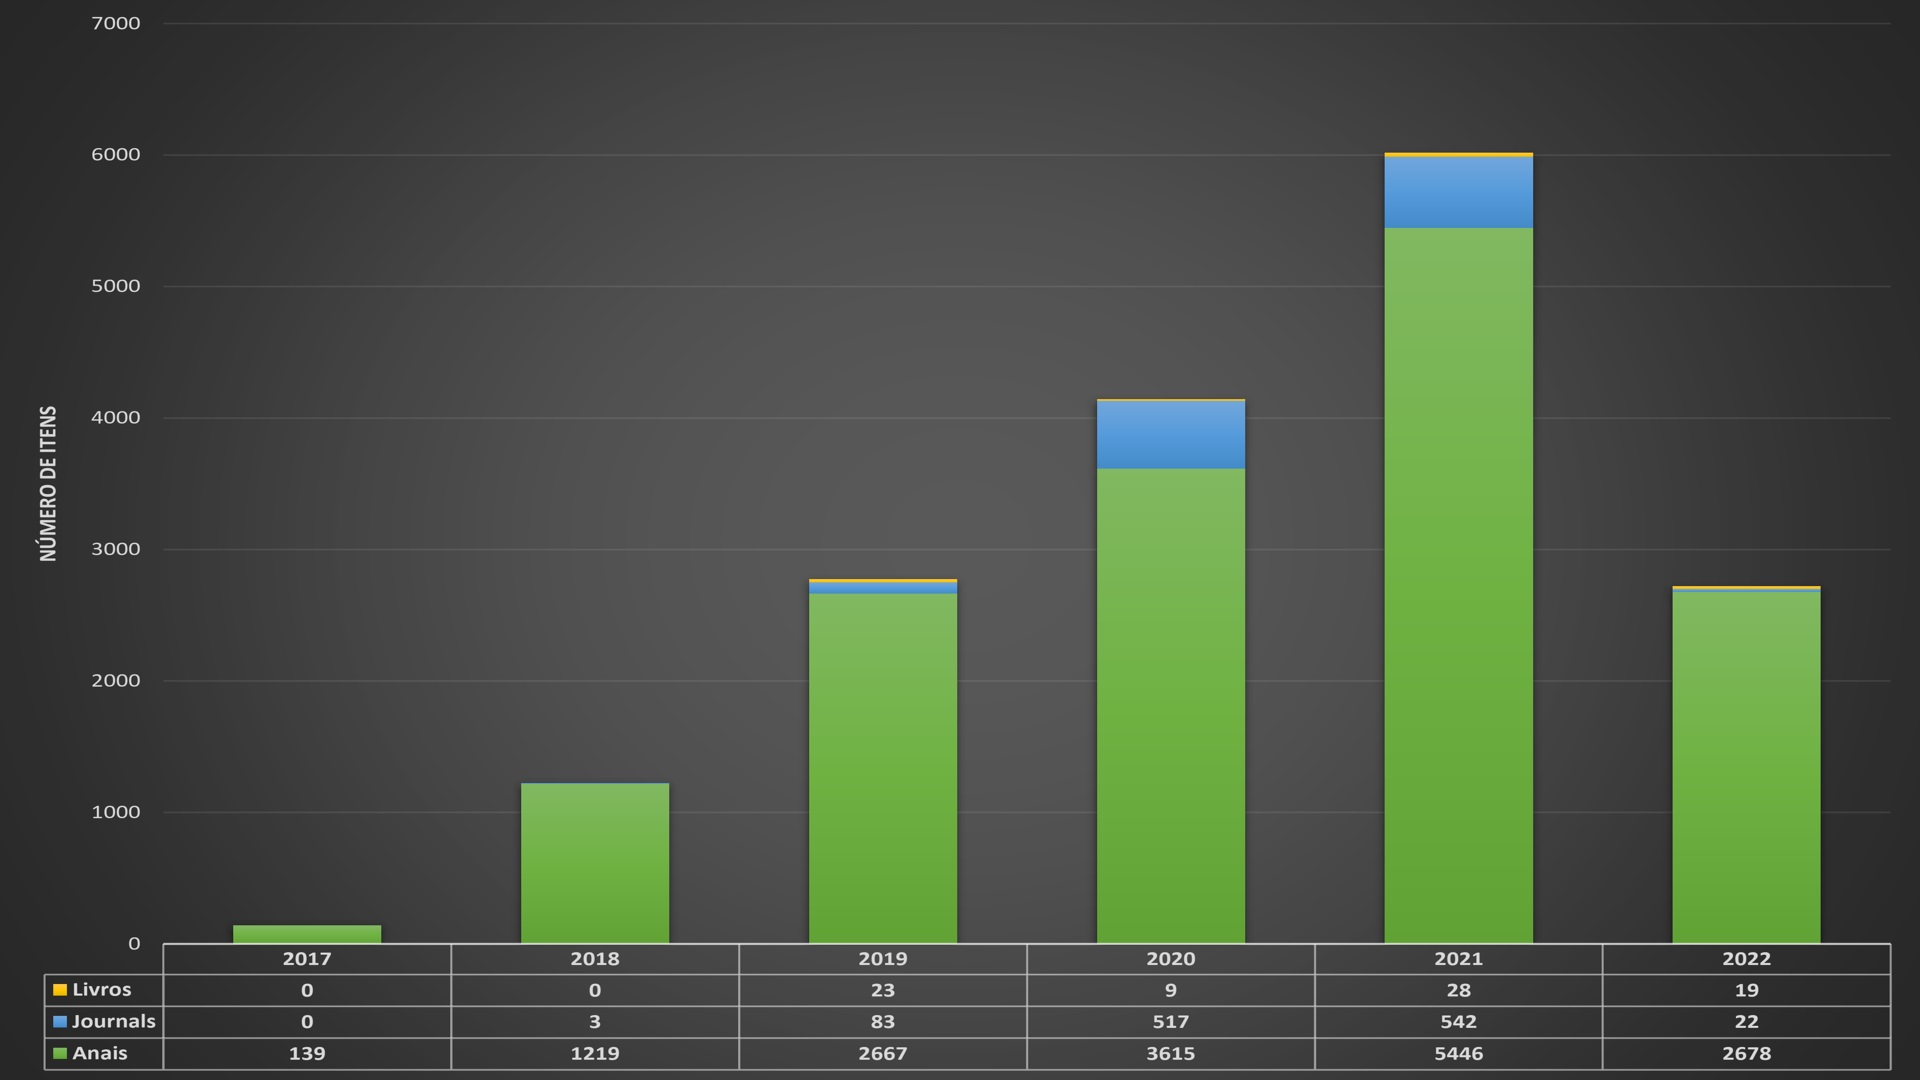
\includegraphics[width=\columnwidth]{sol.jpg}
\caption{Exemplo de legenda de figura.}\label{Fig1}
\end{center}
\end{figure}

Lorem ipsum dolor sit amet, consectetur adipiscing elit, sed do eiusmod tempor incididunt ut labore et dolore magna aliqua. Ut enim ad minim veniam, quis nostrud exercitation ullamco laboris nisi ut aliquip ex ea commodo consequat. Duis aute irure dolor in reprehenderit in voluptate velit esse cillum dolore eu fugiat nulla pariatur. Excepteur sint occaecat cupidatat non proident, sunt in culpa qui officia deserunt mollit anim id est laborum. Lorem ipsum dolor sit amet, consectetur adipiscing elit, sed do eiusmod tempor incididunt ut labore et dolore magna aliqua. Ut enim ad minim veniam, quis nostrud exercitation ullamco laboris nisi ut aliquip ex ea commodo consequat. Duis aute irure dolor in reprehenderit in voluptate velit esse cillum dolore eu fugiat nulla pariatur. Excepteur sint occaecat cupidatat non proident, sunt in culpa qui officia deserunt mollit anim id est laborum.

Lorem ipsum dolor sit amet, consectetur adipiscing elit, sed do eiusmod tempor incididunt ut labore et dolore magna aliqua. Ut enim ad minim veniam, quis nostrud exercitation ullamco laboris nisi ut aliquip ex ea commodo consequat. Duis aute irure dolor in reprehenderit in voluptate velit esse cillum dolore eu fugiat nulla pariatur. Excepteur sint occaecat cupidatat non proident, sunt in culpa qui officia deserunt mollit anim id est laborum. Lorem ipsum dolor sit amet, consectetur adipiscing elit, sed do eiusmod tempor incididunt ut labore et dolore magna aliqua. Ut enim ad minim veniam, quis nostrud exercitation ullamco laboris nisi ut aliquip ex ea commodo consequat. Duis aute irure dolor in reprehenderit in voluptate velit esse cillum dolore eu fugiat nulla pariatur. Excepteur sint occaecat cupidatat non proident, sunt in culpa qui officia deserunt mollit anim id est laborum \textbf{Figure \ref{Fig2}}.

\begin{figure*}
\begin{center}
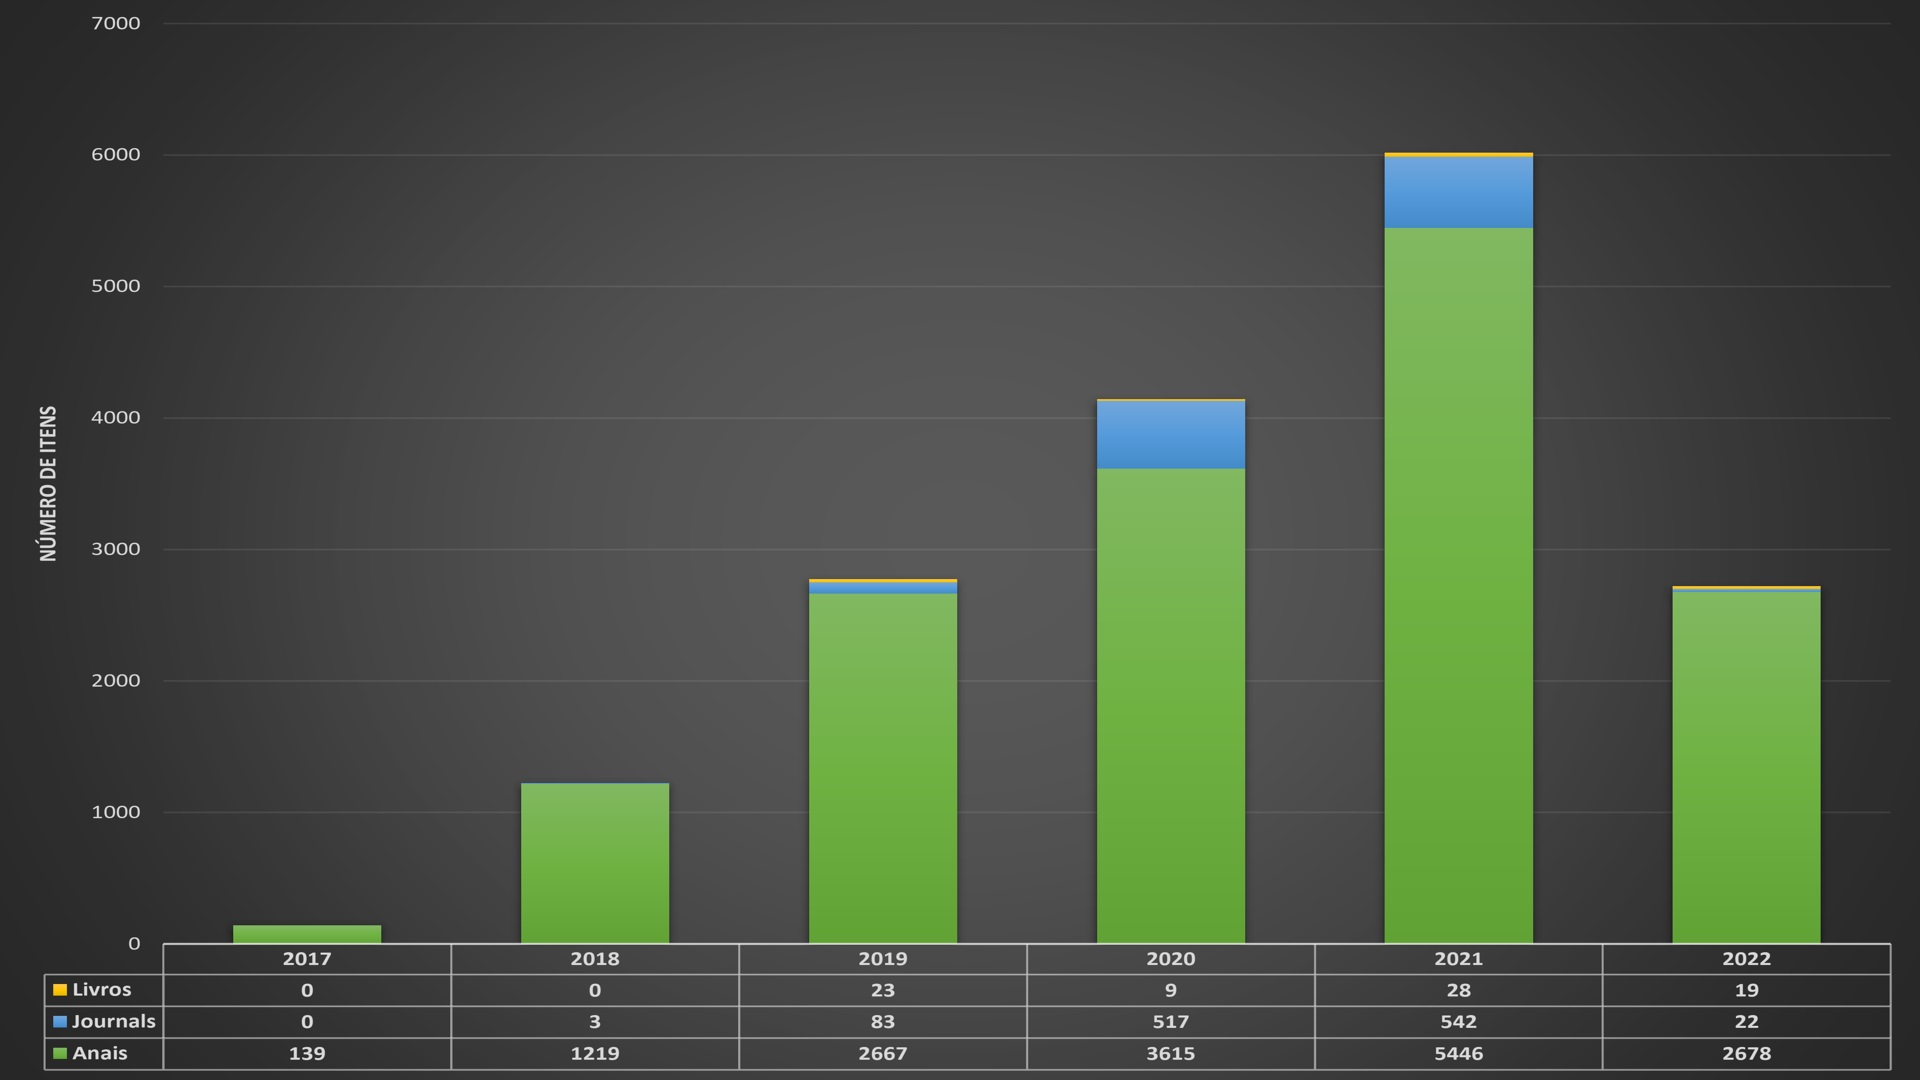
\includegraphics[width=30pc]{sol.jpg}
\caption{{Exemplo de legenda de figura.}}
 \label{Fig2}
\end{center}
\end{figure*}

Lorem ipsum dolor sit amet, consectetur adipiscing elit, sed do eiusmod tempor incididunt ut labore et dolore magna aliqua. Ut enim ad minim veniam, quis nostrud exercitation ullamco laboris nisi ut aliquip ex ea commodo consequat. Duis aute irure dolor in reprehenderit in voluptate velit esse cillum dolore eu fugiat nulla pariatur. Excepteur sint occaecat cupidatat non proident, sunt in culpa qui officia deserunt mollit anim id est laborum. Lorem ipsum dolor sit amet, consectetur adipiscing elit, sed do eiusmod tempor incididunt ut labore et dolore magna aliqua. Ut enim ad minim veniam, quis nostrud exercitation ullamco laboris nisi ut aliquip ex ea commodo consequat. Duis aute irure dolor in reprehenderit in voluptate velit esse cillum dolore eu fugiat nulla pariatur. Excepteur sint occaecat cupidatat non proident, sunt in culpa qui officia deserunt mollit anim id est laborum.

Lorem ipsum dolor sit amet, consectetur adipiscing elit, sed do eiusmod tempor incididunt ut labore et dolore magna aliqua. Ut enim ad minim veniam, quis nostrud exercitation ullamco laboris nisi ut aliquip ex ea commodo consequat. Duis aute irure dolor in reprehenderit in voluptate velit esse cillum dolore eu fugiat nulla pariatur. Excepteur sint occaecat cupidatat non proident, sunt in culpa qui officia deserunt mollit anim id est laborum. Lorem ipsum dolor sit amet, consectetur adipiscing elit, sed do eiusmod tempor incididunt ut labore et dolore magna aliqua. Ut enim ad minim veniam, quis nostrud exercitation ullamco laboris nisi ut aliquip ex ea commodo consequat. Duis aute irure dolor in reprehenderit in voluptate velit esse cillum dolore eu fugiat nulla pariatur. Excepteur sint occaecat cupidatat non proident, sunt in culpa qui officia deserunt mollit anim id est laborum.

Lorem ipsum dolor sit amet, consectetur adipiscing elit, sed do eiusmod tempor incididunt ut labore et dolore magna aliqua. Ut enim ad minim veniam, quis nostrud exercitation ullamco laboris nisi ut aliquip ex ea commodo consequat. Duis aute irure dolor in reprehenderit in voluptate velit esse cillum dolore eu fugiat nulla pariatur. Excepteur sint occaecat cupidatat non proident, sunt in culpa qui officia deserunt mollit anim id est laborum. Lorem ipsum dolor sit amet, consectetur adipiscing elit, sed do eiusmod tempor incididunt ut labore et dolore magna aliqua. Ut enim ad minim veniam, quis nostrud exercitation ullamco laboris nisi ut aliquip ex ea commodo consequat. Duis aute irure dolor in reprehenderit in voluptate velit esse cillum dolore eu fugiat nulla pariatur. Excepteur sint occaecat cupidatat non proident, sunt in culpa qui officia deserunt mollit anim id est laborum.



\paragraph{Exemplo de Título Nível 4.}

Excepteur sint occaecat cupidatat non proident, sunt in culpa qui officia deserunt mollit anim id est laborum. Lorem ipsum dolor sit amet, consectetur adipiscing elit, sed do eiusmod tempor incididunt ut labore et dolore magna aliqua. Ut enim ad minim veniam, quis nostrud exercitation ullamco laboris nisi ut aliquip ex ea commodo consequat. Duis aute irure dolor in reprehenderit in voluptate velit esse cillum dolore eu fugiat nulla pariatur. 

Lorem ipsum dolor sit amet, consectetur adipiscing elit, sed do eiusmod tempor incididunt ut labore et dolore magna aliqua. Ut enim ad minim veniam, quis nostrud exercitation ullamco laboris nisi ut aliquip ex ea commodo consequat. Excepteur sint occaecat cupidatat non proident, sunt in culpa qui officia deserunt mollit anim id est laborum. Lorem ipsum dolor sit amet, consectetur adipiscing elit, sed do eiusmod tempor incididunt ut labore et dolore magna aliqua. Ut enim ad minim veniam, quis nostrud exercitation ullamco laboris nisi ut aliquip ex ea commodo consequat. Duis aute irure dolor in reprehenderit in voluptate velit esse cillum dolore eu fugiat nulla pariatur. Excepteur sint occaecat cupidatat non proident, sunt in culpa qui officia deserunt mollit anim id est laborum.

\section{Conclusão}

Excepteur sint occaecat cupidatat non proident, sunt in culpa qui officia deserunt mollit anim id est laborum. Lorem ipsum dolor sit amet, consectetur adipiscing elit, sed do eiusmod tempor incididunt ut labore et dolore magna aliqua. Ut enim ad minim veniam, quis nostrud exercitation ullamco laboris nisi ut aliquip ex ea commodo consequat. Duis aute irure dolor in reprehenderit in voluptate velit esse cillum dolore eu fugiat nulla pariatur. 

Lorem ipsum dolor sit amet, consectetur adipiscing elit, sed do eiusmod tempor incididunt ut labore et dolore magna aliqua. Ut enim ad minim veniam, quis nostrud exercitation ullamco laboris nisi ut aliquip ex ea commodo consequat. Excepteur sint occaecat cupidatat non proident, sunt in culpa qui officia deserunt mollit anim id est laborum. Lorem ipsum dolor sit amet, consectetur adipiscing elit, sed do eiusmod tempor incididunt ut labore et dolore magna aliqua. Ut enim ad minim veniam, quis nostrud exercitation ullamco laboris nisi ut aliquip ex ea commodo consequat. Duis aute irure dolor in reprehenderit in voluptate velit esse cillum dolore eu fugiat nulla pariatur. Excepteur sint occaecat cupidatat non proident, sunt in culpa qui officia deserunt mollit anim id est laborum \citep{ref5}.


\begin{declarations}

\begin{acknowledgements}
ESTA DECLARAÇÃO É OPCIONAL. Este é um texto de agradecimentos com várias linhas. Lorem ipsum dolor sit amet, consectetur adipiscing elit, sed do eiusmod tempor incididunt ut labore et dolore magna aliqua. Ut enim ad minim veniam, quis nostrud exercitation ullamco laboris nisi ut aliquip ex ea commodo consequat.
\end{acknowledgements}


\begin{funding}
ESTA DECLARAÇÃO É OPCIONAL. Esta pesquisa foi financiada por lorem ipsum dolor sit amet, consectetur adipiscing elit.
\end{funding}

\begin{contributions}
ESTA DECLARAÇÃO É OBRIGATÓRIA. 
\textit{Considerar o Código de Conduta da SBC.
Participação em autoria: espera-se que todos os autores de um trabalho publicado 
ou submetido para publicação, tenham tido efetiva participação no respectivo trabalho.}
Sugerimos que os autores descrevam sua contribuição usando 
a Taxonomia CRediT (\href{https://credit.niso.org/}{https://credit.niso.org/}) como neste exemplo: 
JV contribuiu para a concepção deste estudo. CB, RP e CM realizaram os experimentos. 
JV é o principal contribuidor e escritor deste manuscrito. 
Todos os autores leram e aprovaram o manuscrito final. 
\end{contributions}

\begin{interests}
ESTA DECLARAÇÃO É OBRIGATÓRIA. 
Se não houver conflitos de interesse, os autores devem declarar: 
``Os autores declaram que não têm nenhum conflito de interesses''. 
Caso contrário, a declaração deve ser: 
``Os autores declaram que têm os seguintes conflitos de interesses: 
lorem ipsum dolor sit amet, consectetur adipiscing elit.''
\end{interests}

\begin{materials}
ESTA DECLARAÇÃO É OBRIGATÓRIA. 
\textit{Considerar o Código de Conduta da SBC. 
Reprodutibilidade de resultados de pesquisa: 
nos casos pertinentes, recomenda-se que artigos indiquem 
a disponibilidade pública de material utilizado nas revisões, 
de modo a facilitar a reprodução dos respectivos resultados por outros pesquisadores.}
%
Se os autores disponibilizaram seus dados e/ou códigos abertamente, a declaração deve ser: 
``Os dados e outros materiais criados e/ou usados nesta revisão da literatura
estão disponíveis em \ldots''. 
Caso contrário, a declaração deve ser: 
``Os dados e outros materiais criados e/ou usados nesta revisão da literatura 
serão disponibilizados mediante solicitação''. 
%
Todo o material suplementar disponibilizado publicamente pelos autores aparecerá 
na página de publicação do artigo em caso de aceitação. 
\end{materials}

\begin{aitools}
ESTA DECLARAÇÃO É OBRIGATÓRIA.  
\textit{Considerar o Código de Conduta da SBC.
Uso de Inteligência Artificial (IA) Generativa: 
a utilização de ferramentas e tecnologias de IA Generativa para geração de conteúdos, 
na escrita e/ou revisão do conteúdo de artigos, deve ser declarada explicitamente no trabalho.} 
A declaração deve ocorrer nesta seção, definida especificamente para este fim.
Deve-se listar as ferramentas (e suas versões) e descrever onde foram empregadas, por exemplo, 
textos, tabelas, gráficos, citações, etc. 
Essas ferramentas \textbf{não} podem ser listadas como autores de um artigo. 
O uso de tais ferramentas não exime os autores da responsabilidade 
sobre todo o seu conteúdo, inclusive no caso de ser identificado plágio.
%
Se os autores não utilizaram tais ferramentas, a declaração deve ser: 
``Os autores não utilizaram ferramentas de IA generativa no desenvolvimento do estudo''.
%
\end{aitools}

\begin{furtherinformation}
Manuscritos devem indicar explicitamente como as questões éticas da pesquisa foram abordadas e gerenciadas, 
incluindo a aprovação da pesquisa por um comitê de ética, quando aplicável.
\end{furtherinformation}

\end{declarations}

\bibliographystyle{apalike-sol}
\bibliography{refs}

\end{document}

